% !TeX root = ../main.tex

\chapter{Background}\label{chapter:Background}


This chapter explores the different levels of ECU virtualization, examining the advantages and disadvantages of each and identifying the most effective scenarios for their application. The latest virtualization techniques will be discussed, particularly their application in Real-Time Operating Systems (RTOS). Additionally, some promising software projects will be introduced as potential solutions for ECU virtualization in the case study. The goal of this chapter is to provide a solid understanding of the key concepts and tools essential for the thesis.

\section{vECU Classification}
The simulation of ECUs as virtual ECUs (vECUs) has quickly become integral in various stages of automotive development. Broadly, vECUs can be classified into two main categories: host compiled and target compiled \cite{synopsys2023software}.

Host compiled vECUs do not simulate the ECU hardware itself. Instead, they simulate Application Programming Interfaces (APIs) at key points in the software stack, effectively removing the need for lower, hardware-dependent layers. This means that the vECU does not run the complete production code, and certain layers must be modified. These modifications involve substituting specific software layers, not included in the system under test (SUT), with their simulated counterparts.

In contrast, target compiled vECUs use detailed hardware simulation models to accurately represent the ECU hardware. This enables the production software to run without requiring any alterations, as it is compiled exactly as it would be for the physical ECU used in a vehicle. To achieve this, detailed hardware modeling of the entire ECU is necessary, including its MCUs, internal CPU cores, components, and even board-level devices.

Dependent on the vECU content, different vECU levels can be distinguished. The following outlines an approach for defining and naming vECU layers \cite{smartse2020}, as depicted in ~\autoref{fig:levels}.
\begin{figure}[htpb]
  \centering
  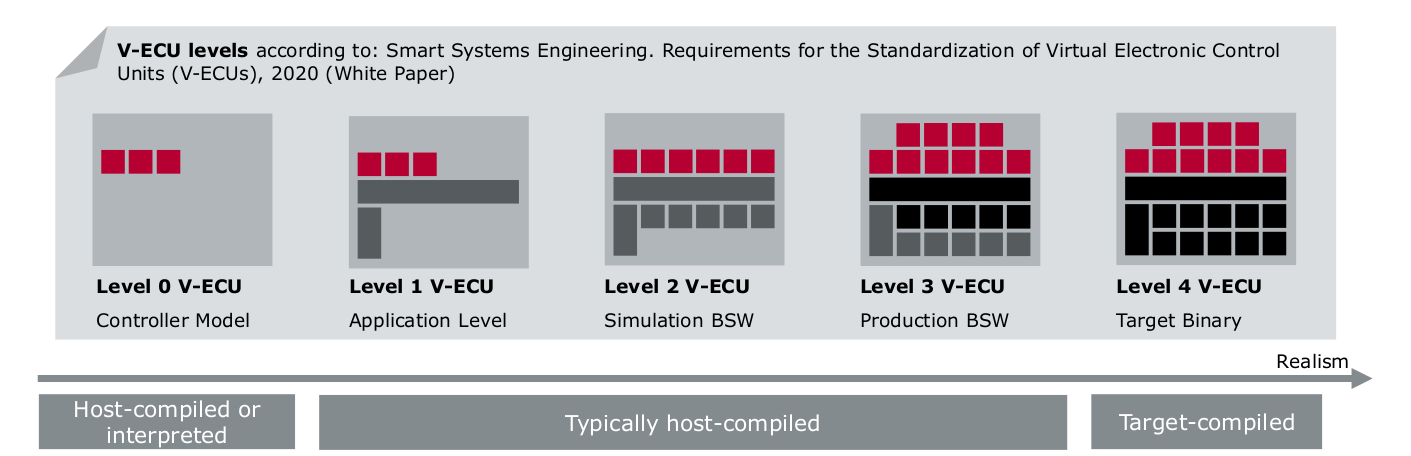
\includegraphics[width=1\textwidth]{figures/levels}
  \caption{Virtual ECU abstraction levels \cite{wenzler2023}.} \label{fig:levels}
\end{figure}

\subsection{Level 0}
The most basic form of ECU virtualization is the Level 0 vECU, which consists solely of the controller model. This model could be represented in various forms, such as a MATLAB Simulink model or C code derived from it. Importantly, this level of virtualization does not include any production code or basic software layers. As a result, Level 0 vECUs are limited to testing the control algorithms themselves and are not suitable for more comprehensive tests, such as software interface tests, which require more advanced types of vECUs closer to the actual production environment.

\subsection{Level 1}
Moving up in complexity, a Level 1 vECU includes the production code of the application software. However, to function correctly in a simulation environment, it requires additional functionalities from lower software layers. These supplementary layers are typically not from the production code but are specifically created or generated for the vECU. In AUTOSAR systems, for example, this would involve the Run-Time Environment (RTE) and the Operating System, along with other functionalities that enable the vECU to handle data transmission and reception. At this level, vECUs are primarily used for testing application functionalities, especially when these functionalities are distributed across multiple components or ECUs. However, they communicate only at the signal level and do not support bus or network communication.

\subsection{Level 2}
Level 2 V-ECUs add another layer of sophistication by incorporating simulated basic software (BSW) functionalities on top of the Level 1 components. Although these BSW functionalities are specifically created for simulation purposes and are not production-level, they enable more extensive testing capabilities. For instance, Level 2 vECUs can handle communication at the bus or network level, such as via simulated CAN or Ethernet, making them suitable for broader application software testing, including bus monitoring and diagnostic tests.

\subsection{Level 3}
At Level 3, vECUs include not only production application software but also production-level basic software (BSW), or in some cases, just the BSW or parts of it, depending on the testing requirements. The application and basic software at this level must be hardware-independent, such as everything above the microcontroller abstraction layer (MCAL) in AUTOSAR systems. While production BSW can be supplemented with simulated components for vECU purposes, the primary goal is to include as much of the real ECU's production code as possible. Level 3 vECUs are versatile, allowing for comprehensive testing of hardware-independent software, testing of networked vECUs, and even serving as rest bus models in hardware-in-the-loop (HIL) tests.

\subsection{Level 4}
The most advanced type of vECU, Level 4, includes the full production code compiled for the actual target ECU, including any hardware dependencies. This allows for a highly accurate simulation that mirrors the real ECU environment. To execute a Level 4 vECU on a simulation platform, an instruction set simulator is necessary, along with a detailed model of the ECU hardware. This level is particularly useful for testing scenarios that depend on the hardware architecture, such as evaluating the computational load of multicore ECUs. An example of level 4 vECU is the VDK from Synopsys \cite{synopsys_aurix_vdk_2020}. \\

To conclude, after evaluating the different levels of ECU virtualization, it becomes evident that Level 3 vECUs present the most suitable choice for implementation in this thesis. This level offers a balanced approach by including as much hardware-independent production code as possible without involving any physical hardware. By incorporating both the application software and the production basic software (BSW) while maintaining hardware independence, Level 3 vECUs allow for comprehensive testing and simulation. This makes them ideal for the scope of this research, where the focus is on maximizing software accuracy and functionality in a virtual environment.

\section{RTOS Simulation}\label{sec:RTOS}
When reviewing modern virtualization techniques, it is apparent that Real-Time Operating Systems (RTOS) virtualization shares many similarities with the level 3 virtualization discussed earlier.
This virtualization allows developers to run and test RTOS applications on a Linux environment, facilitating development and debugging processes without needing physical embedded hardware. Examples of RTOS platforms relevant to AUTOSAR standards include FreeRTOS, ThreadX, and Zephyr. These platforms are designed for applications that require precise timing and high reliability, making them suitable for use in automotive embedded systems.  
 
\subsection{Key Components of RTOS Simulation}
Several key components of an RTOS are emulated using the host OS features. These components include task management, the scheduler, interrupt handling, and timers.
\begin{enumerate}

\item \textbf{Task Management:} On actual hardware, tasks are managed using hardware-specific context-switching mechanisms. In simulation, tasks are represented as threads in the host OS, such as POSIX threads on Linux.

\item \textbf{Scheduler:} The scheduler in an RTOS is responsible for managing task priorities and context switching based on timing and event triggers. This functionality is emulated in software during simulation. The scheduler maintains the same logic for task prioritization and preemption, using host OS mechanisms to switch between threads.

\item \textbf{Interrupt Handling:} Hardware interrupts are critical in real-time systems for immediate response to events. These interrupts are serviced by specific interrupt service routines (ISRs). In a simulated environment, interrupts are emulated using host OS signals or inter-thread communication methods, creating handlers that mimic the behavior of ISRs.

\item \textbf{Timers:} RTOS relies heavily on hardware timers to trigger periodic tasks and manage timeouts. In simulation, host OS timers are used to replicate this functionality. For example, Linux system calls such as “setitimer” or “timer\_create” generate timer signals that simulate the periodic interrupts.
\end{enumerate}

\subsection{Simulation in Threadx}
ThreadX for Linux simulates an RTOS environment by utilizing POSIX pthreads to represent RTOS tasks and the scheduler. ~\autoref{fig:threads} gives an overview of the key implementation aspects \cite{threadx_readme}:
\begin{enumerate}
\item \textbf{Thread Representation: }
In the ThreadX simulation, each RTOS task is mapped to a POSIX pthread. When an application thread is created using the ThreadX API (e.g., tx\_thread\_create), a corresponding pthread is instantiated. These pthreads perform the same functions as their RTOS counterparts, allowing developers to test and debug real-time applications in a simulated environment.
\item \textbf{Scheduler Implementation: } 
The ThreadX scheduler is implemented as a high priority pthread. This scheduler thread determines which application thread to run based on their priorities and states. The scheduler preempts lower-priority threads to ensure that the highest-priority thread is always executing, mimicking the behavior of the RTOS on actual hardware.
\item \textbf{Simulated Interrupts: }
Simulated interrupts are handled using POSIX mechanisms such as signals. Interrupt Service Routines (ISRs) in ThreadX are mapped to signal handlers in Linux. When an interrupt is simulated, a signal is sent to the appropriate pthread, invoking the ISR. This allows the simulation to handle interrupts similarly to an actual RTOS.
\item \textbf{Timer Management: }
Timers in ThreadX are implemented using Linux system timers. Functions like "\textbf{setitimer}" or "\textbf{timer\_create}" generate periodic events, triggering timer-related tasks in the application. This ensures that timing behavior in the simulation is accurate and consistent with real-time requirements.
\end{enumerate}
\begin{figure}[htpb]
  \centering
  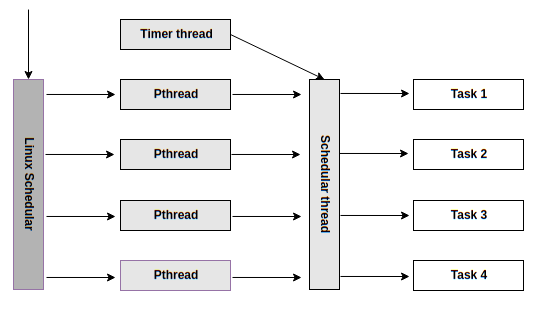
\includegraphics[width=0.8\textwidth]{figures/threads2}
  \caption{RTOS simulation on Linux.} \label{fig:threads}
\end{figure}


\subsection{Simulation in FreeRTOS}
The virtualization in FreeRTOS for Linux is achieved through a combination of Linux pthreads, mutexes, condition variables, and high-resolution timers. Here is a breakdown of how these elements are integrated \cite{freertos_simulator}:
\begin{enumerate}
\item \textbf{Pthreads for Task Management: }
Each FreeRTOS task is implemented as a pthread, allowing the FreeRTOS kernel to create, manage, and delete tasks in a manner analogous to its operation on embedded hardware.
\item \textbf{Condition Variables for Synchronization: }
FreeRTOS's synchronization primitives such as semaphores and queues are mapped to condition variables and mutexes in Linux. This mapping ensures that tasks can synchronize correctly even in a simulated environment.
\item \textbf{High-Resolution Timers for Tick Simulation: }
A dedicated high-priority thread generates periodic tick interrupts, simulating the hardware timer interrupts that FreeRTOS relies on. This thread sleeps for a specified interval (configurable to match the tick rate) and then signals the FreeRTOS scheduler to perform context switching and other periodic operations.
\item \textbf{Interfacing with Linux I/O: }
While the FreeRTOS simulator is running, it uses standard Linux system calls for I/O operations such as reading from and writing to the console. This makes it easier to debug and monitor the behavior of FreeRTOS tasks and system calls.
\end{enumerate}

\subsection{Simulation in Zephyr}
similar to ThreadX and FreeRTOS, Zephyr also provides a simulation environment that facilitates development and testing on host systems without the need for embedded hardware. This is achieved by virtualizing key components of the RTOS, leveraging the host operating system's features. Zephyr's simulation environment, particularly its native POSIX port, uses POSIX threads and system calls to emulate the behavior of the Zephyr kernel. \cite{zephyr_native_simulator}

\subsection{Benefits and Challenges of RTOS Simulation}
Simulation of RTOS offers several benefits. It is cost-effective as there is no need for physical hardware during the initial development phase. It is also flexible, allowing easy modification and testing of different configurations and scenarios. Additionally, it provides enhanced debugging capabilities using host OS tools, which can be more sophisticated than those available for embedded hardware.
While RTOS simulation provides a valuable platform for development and testing, it is important to acknowledge its limitations:
\begin{enumerate}
\item \textbf{Non-Real-Time Behavior: } The simulator runs on a general-purpose Linux operating system, which does not guarantee real-time behavior. Therefore, timing accuracy and real-time performance cannot be ensured.
\item \textbf{System Call Overheads: } Console I/O and other Linux system calls can interfere with the RTOS simulation, potentially affecting task execution and timing.
\item \textbf{Hardware-Specific Features: } Certain hardware-specific features and peripherals cannot be accurately emulated in the simulation environment.
\end{enumerate}